% Created 2021-02-11 jue 12:00
% Intended LaTeX compiler: pdflatex
\documentclass[presentation,aspectratio=169]{beamer}
\usepackage[utf8]{inputenc}
\usepackage[T1]{fontenc}
\usepackage{graphicx}
\usepackage{grffile}
\usepackage{longtable}
\usepackage{wrapfig}
\usepackage{rotating}
\usepackage[normalem]{ulem}
\usepackage{amsmath}
\usepackage{textcomp}
\usepackage{amssymb}
\usepackage{capt-of}
\usepackage{hyperref}
\usepackage{khpreamble}
\usepackage{amssymb}
\usepgfplotslibrary{groupplots}
\newcommand*{\shift}{\operatorname{q}}
\usetheme{default}
\author{Kjartan Halvorsen}
\date{2021-02-11}
\title{Diagrama de bloques}
\hypersetup{
 pdfauthor={Kjartan Halvorsen},
 pdftitle={Diagrama de bloques},
 pdfkeywords={},
 pdfsubject={},
 pdfcreator={Emacs 26.3 (Org mode 9.4.4)}, 
 pdflang={English}}
\begin{document}

\maketitle

\section{Recap}
\label{sec:orgc132a6a}
\begin{frame}[label={sec:org7ae6403}]{Sistemas mecatrónicos}
\begin{center}
\includegraphics[height=0.7\textheight]{../../figures/ac75.jpeg}\\
{\footnotesize  From SailingWorld}
\end{center}

\href{https://www.sailingscuttlebutt.com/wp-content/uploads/2018/03/AC75\_Class\_Rule.pdf}{AC75 Class rule}
\end{frame}


\begin{frame}[label={sec:org0609b2a}]{sistema de hidroalas}
 \begin{center}
\includegraphics[height=0.6\textheight]{../../figures/ac75-lines.png}
\includegraphics[height=0.7\textheight]{../../figures/ac75-class-foil.png}\\
{\footnotesize  by françois chevalier \hfill from the ac75 class rule}
\end{center}
\end{frame}

\section{Control lazo abierto, lazo cerrado}
\label{sec:orgdf36917}

\begin{frame}[label={sec:org1ff1759}]{Qué es \alert{control en lazo abierto} y \alert{en lazo cerrado}?}
\begin{block}{Lazo abierto: \alert{No} existe retroalimentación de señales medidas}
\begin{center}
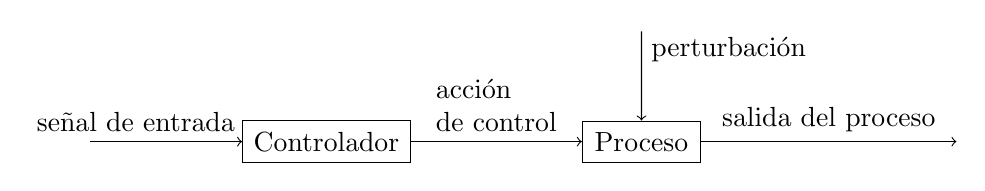
\begin{tikzpicture}[scale=0.6, node distance=22mm, block/.style={rectangle, draw, minimum width=15mm, inner sep=4pt}, sumnode/.style={circle, draw, inner sep=2pt}]

  \node[coordinate] (input) {};
  \node[block, right of=input, node distance=30mm] (fb)  {Controlador};
  \node[block, right of=fb, node distance=40mm] (plant)  {Proceso};

  \node[coordinate, above of=plant, node distance=14mm] (disturbance) {};
  \node[coordinate, right of=plant, node distance=40mm] (output) {};

  \draw[->] (input) -- node[above, pos=0.3] {señal de entrada} (fb);
  \draw[->] (fb) -- node[above, align=left,] {acción \\de control} (plant);
  \draw[->] (plant) -- node[coordinate] (meas) {} node[above,] {salida del proceso} (output);
  \draw[->] (disturbance) -- node[right, pos=0.2] {perturbación} (plant);
\end{tikzpicture}
\end{center}
\end{block}
\end{frame}

\begin{frame}[label={sec:org63c2010}]{Qué es \alert{control en lazo abierto} y \alert{en lazo cerrado}?}
\begin{block}{Lazo abierto: \alert{No} existe retroalimentación de señales medidas}
\begin{center}
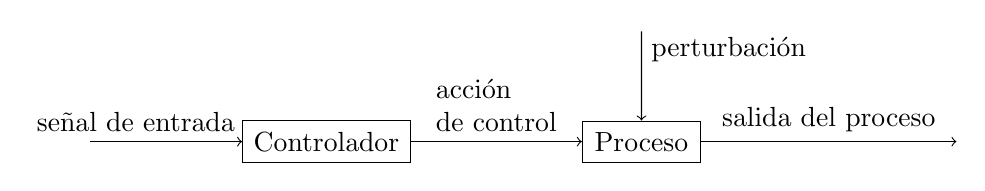
\begin{tikzpicture}[scale=0.6, node distance=22mm, block/.style={rectangle, draw, minimum width=15mm, inner sep=4pt}, sumnode/.style={circle, draw, inner sep=2pt}]

  \node[coordinate] (input) {};
  \node[block, right of=input, node distance=30mm] (fb)  {Controlador};
  \node[block, right of=fb, node distance=40mm] (plant)  {Proceso};

  \node[coordinate, above of=plant, node distance=14mm] (disturbance) {};
  \node[coordinate, right of=plant, node distance=40mm] (output) {};

  \draw[->] (input) -- node[above, pos=0.3] {señal de entrada} (fb);
  \draw[->] (fb) -- node[above, align=left,] {acción \\de control} (plant);
  \draw[->] (plant) -- node[coordinate] (meas) {} node[above,] {salida del proceso} (output);
  \draw[->] (disturbance) -- node[right, pos=0.2] {perturbación} (plant);
\end{tikzpicture}
\end{center}
\end{block}


\begin{block}{Lazo cerrado: Elimina o compensa efecto de perturbaciones}
\begin{center}
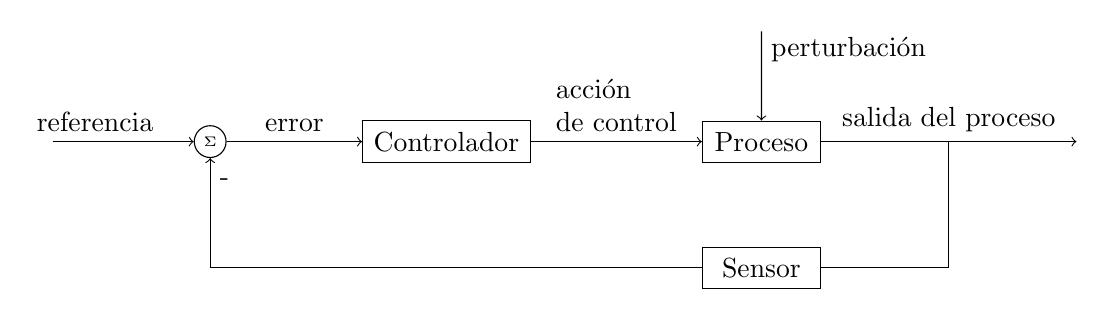
\begin{tikzpicture}[scale=0.6, node distance=22mm, block/.style={rectangle, draw, minimum width=15mm, inner sep=4pt}, sumnode/.style={circle, draw, inner sep=2pt}]

  \node[coordinate] (input) {};
  \node[sumnode, right of=input, node distance=20mm] (sumerr) {\tiny $\Sigma$};
  \node[block, right of=sumerr, node distance=30mm] (fb)  {Controlador};
  \node[block, right of=fb, node distance=40mm] (plant)  {Proceso};
  \node[block, below of=plant, node distance=16mm] (sensor)  {Sensor};

  \node[coordinate, above of=plant, node distance=14mm] (disturbance) {};
  \node[coordinate, right of=plant, node distance=40mm] (output) {};

  \draw[->] (input) -- node[above, pos=0.3] {referencia} (sumerr);
  \draw[->] (sumerr) -- node[above] {error} (fb);
  \draw[->] (fb) -- node[above, align=left,] {acción \\de control} (plant);
  \draw[->] (plant) -- node[coordinate] (meas) {} node[above,] {salida del proceso} (output);
  \draw[->] (disturbance) -- node[right, pos=0.2] {perturbación} (plant);
  \draw[->] (meas) |- (sensor) -| node[right, pos=0.9] {-} (sumerr);
\end{tikzpicture}
\end{center}
\end{block}
\end{frame}

\begin{frame}[label={sec:org2cd7a65}]{Control en lazo abierto}
\begin{center}
\includegraphics[width=0.7\textwidth]{../../figures/ac75-control-no-actuator}
\end{center}
\end{frame}

\begin{frame}[label={sec:org985a671}]{Control en lazo abierto}
\begin{center}
\includegraphics[width=0.99\textwidth]{../../figures/ac75-control-no-control}
\end{center}
\end{frame}

\begin{frame}[label={sec:org3e0c2a1}]{Control en lazo abierto}
\begin{center}
\includegraphics[width=1.0\textwidth]{../../figures/ac75-control-block}
\end{center}
\end{frame}

\begin{frame}[label={sec:org5c0a2a4}]{Control en lazo cerrado}
\begin{center}
\includegraphics[width=1.0\textwidth]{../../figures/ac75-control-block-feedback}
\end{center}
\end{frame}



\begin{frame}[label={sec:org7fee771}]{Control en lazo cerrado}
\begin{center}
\includegraphics[width=1.02\textwidth]{../../figures/ac75-control-block-outer-feedback}
\end{center}

Retroalimentación del \emph{yacht state} \alert{no} permisible.
\end{frame}


\section{Block diagram}
\label{sec:org4554415}

\begin{frame}[label={sec:org5212a7f}]{El diagrama de bloque describe \alert{flujo de señales}}
\begin{center}
\includegraphics[width=1.0\textwidth]{../../figures/ac75-control-block-feedback-units}
\end{center}
\end{frame}


\begin{frame}[label={sec:org102fd58}]{El diagrama de bloque describe \alert{flujo de señales}}
\begin{center}
\includegraphics[width=.8\textwidth]{../../figures/ac75-control-block-feedback-units}
\end{center}


\begin{itemize}
\item El \alert{actuador} convierte una señal de información a fuerza/torque/flujo/energía
\item El \alert{sensor} convierte un variable físico a una señal de información
\end{itemize}
\end{frame}
\end{document}